\twocolumn
    \begin{doublespace}
        \textbf{3.} \((x + 1)\Big[\big(\frac{1}{2}\big)^{2(x-1)} + 11\big(\frac{1}{2}\big)^{x}\Big]-3=0; \\ x_1=-1;\qquad \big(\frac{1}{2}\big)^{x}=y;\qquad 4y^{2} + 11y -3=\\=0;\quad y_1=\frac{1}{4};\qquad y_2=-3<0;\qquad \big(\frac{1}{2}\big)^{x}=\\=\big(\frac{1}{2}\big)^{2};\qquad x_2=2;\)
        Около 70\% абитуриентов не указали корень \(x=-1\).
    \end{doublespace}\par
    \begin{doublespace}
        \textbf{4.} Так как при \(\frac{\pi}{2} \leq x \leq \frac{3\pi}{2}\) имеем \(\cos{x} \leq 0\), то
        \[\sqrt{1-\sin^2{x}}=-\cos{x},\]
        \[8\cos^2{x} - 2\cos{x} -3 =0,\]
        \[\cos{x}=-\frac{1}{2},\]
        \[x_1=\frac{2}{3}\pi,\quad x_2=\frac{4}{3}\pi.\]
    \end{doublespace}\par
    Некоторые абитуриенты уединяли радикал и возводили обе части уравнения в квадрат. Другие не учитывали области определения аргумента и писали
    \[x=\pm\frac{2}{3}\pi + 2k\pi.\]\par
    \begin{center}
    \subsubsection*{Финансовый факультет}
    \end{center}\par
    \textbf{1.} Задача допускает несколько интересных решений с использованием теоремы синусов, теоремы тангенсов, с приминением дополнительных построений и др. Приведем одно из них (рис. 3):
    \[\tan{2\alpha}=\frac{3a}{h},\quad 3\tan{\alpha}=\frac{3a}{h},\quad \tan{2\alpha}=3\tan{\alpha},\]
    \[\frac{2\tan{\alpha}}{1-\tan^2{\alpha}}=3\tan{\alpha}, \quad \tan{\alpha}=\frac{\sqrt{3}}{3}, \quad \alpha=30^\circ.\]\par
    Ответ: AB = 10 \textit{см}, AC = 20 \textit{см}, BC = \(10\sqrt{3}\). \par
    \begin{onehalfspace}
    \textbf{2. }
         \(\quad \lg^2{2x} + \lg^2{3x} = \lg^2{2} + \lg^2{3},\)
    \[\lg^2{2x} - \lg^2{2}= \lg^2{3} - \lg^2{3x},\]
    \[\lg{x} \cdot \lg{4x}=\lg{\frac{1}{x}} \cdot \lg{9x} = - \lg{x} \cdot \lg{9x}.\]\par
    1) \(\lg{x}=0, \quad x_1 = 1\); \par
    2) \(\lg{4x} = - \lg{9x}\),
    \[\lg{4} + \lg{x} + \lg{9} + \lg{x} = 0,\]
    \[2\lg{x} = -\lg{36}, \quad x^2 = \frac{1}{36}, \quad x_2 = \frac{1}{6}.\]\par
    \end{onehalfspace}
    \textbf{3. } Составим таблицу:\par
    \begin{center}
        \begin{tabular}{|c|c|c|c|c|c|}
            \hline
            \parbox[b]{0.95 cm}{\begin{center}\scriptsize Авто-\\мобили\end{center}} & \parbox[b]{0.8 cm}{\begin{center}\scriptsizeСко-\\рость\end{center}} & \rotatebox{90}{\parbox{1.8 cm}{\scriptsizeВремя дви-\\жения до\\встречи}} & \rotatebox{90}{\parbox{1.8 cm}{\scriptsizeПройденное\\расстояние\\до встречи}} & \rotatebox{90}{\parbox{1.8 cm}{\scriptsizeПройденное\\расстояние\\после встре-\\чи}} & \rotatebox{90}{\parbox{1.8 cm}{\scriptsizeВремя дви-\\жения после\\встречи}} \\ 
            \hline
            I & x & 4 & 4x & 4y & \parbox[c][0.7 cm]{1 cm}{\begin{center}\(4\frac{y}{x}\)\end{center}} \\
            \hline
            II & y & 4 & 4y & 4x & \parbox[c][0.7 cm]{1 cm}{\begin{center}\(4\frac{x}{y}\)\end{center}} \\
            \hline
        \end{tabular}
    \end{center}\par
    \begin{center}
    \begin{rcases}
        \(4x + 4y = 280,\)\\
        \(4\frac{y}{x} - 4\frac{x}{y} = \frac{7}{3},\)
    \end{rcases}
    \(\frac{y}{x} = t;\)
    \end{center}
    \[4t - \frac{4}{t} = \frac{7}{3}, \quad 12t^2 - 7t - 12=0;\]
    \[t = \frac{4}{3}; \quad y = \frac{4}{3}x; \quad x = 30 \quad \textit{км/ч},\]
    \[y = 40 \quad \textit{км/ч}.\]\par
    \textbf{4. } \(\quad \sin{x}\cdot\sin{2x}\cdot\sin{3x} = \frac{1}{4}\sin{4x},\)
    \[4\sin{x}\cdot\sin{2x}\cdot\sin{3x} = 2\sin{2x}\cos{2x},\]
    \[\sin{2x}(2\sin{x}\sin{3x} - \cos{2x})=0,\]
    \[\sin{2x}(\cos{2x} - \cos{4x} - \cos{2x})=0,\]
    \[\sin{2x}\cos{4x}=0,\]
    \[x=\frac{k\pi}{2}, \quad x= \frac{\pi}{8}(2k+1) \quad (k=0, \quad \pm1,\]
    \begin{flushright}
        \(\pm2,\quad\dots)\)
    \end{flushright}
    \begin{center}
    \subsubsection*{Факультет товароведения промышленных товаров}
    \end{center}\par
    \begin{doublespace}
    \textbf{1.} 14 \textit{км/ч}, 2\textit{км/ч}.\par
    \textbf{2.} \(\frac{2}{\pi}\cdot\frac{\sin{\alpha} + \sin{\beta}}{\sin{\alpha}\cdot\cos{\beta}}\).\par
    \textbf{3.} \(x=2\).\par
    \textbf{4.} Решений нет.\par
    \end{doublespace}\par
    \begin{center}
    \subsubsection*{Факультет экономики и организации материально-технического снабжения}
    \end{center}\par
    \begin{doublespace}
    \textbf{1.} \(2<x<3; \quad 6<x<7\).\par
    \textbf{2.} \(V=\frac{2}{3}h^3\sin{\alpha}\tan^2{\varphi}\sin{\alpha+\beta}\sin{\beta}\) \textit{куб. ед}.\par
    \textbf{3.} 6 \textit{км/ч}, 4 \textit{км/ч}, 10 \textit{км}.\par
    \textbf{4.} \(x=\pi k; \quad (-1)^{x}\arcsin{\frac{3}{4}} + \pi k.\).\par
    \end{doublespace}
    \begin{center}
    \subsubsection*{Факультет экономики промышленности}
    \end{center}\par
    \begin{onehalfspace}
    \textbf{1. } 80 \textit{км/ч}, 48\textit{км/ч}, 480\textit{км}.\par
    \textbf{2. } \(V=\frac{2\sqrt{3}}{3\cdot35}H^3; \quad S=\frac{2\sqrt{3}}{5}H^2\).\par
    \textbf{3. } \(x=3\).\par
    \textbf{4. } \(x=\frac{\pi}{6} + \pi k\).\par
    \end{onehalfspace}\par
    \begin{center}
    \subsubsection*{Торгово-экономичемский факультет}
    \end{center}\par
    \begin{onehalfspace}
    \textbf{1. } \(x=2\).\par
    \textbf{2. } \(V=\frac{2}{3}a^3\cos{\frac{\alpha}{2}}\tan{\varphi}\).\par
    \textbf{3. } \(x=3\).\par
    \textbf{4. } \(x=\frac{\pi}{6} + \pi k\).\par
    \end{onehalfspace}
    \begin{flushleft}
    \subsubsection*{К заметке "<Наш зоопарк">}
    \end{flushleft}\par
    \begin{center}
    \textit{(см. "<Квант"> № 1, 1973)}
    \end{center}
    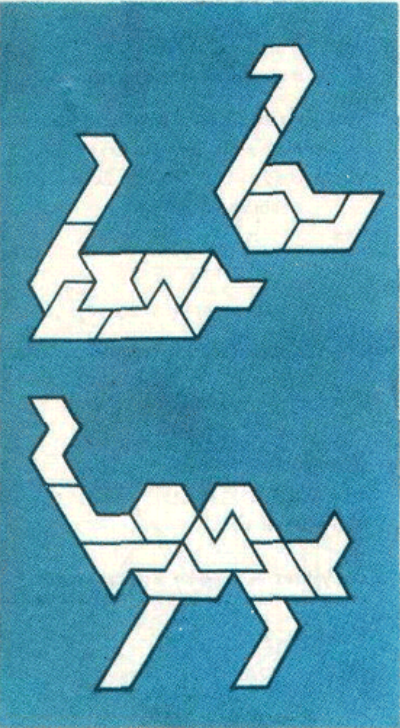
\includegraphics{img.png}
    